\section{Computer architectures}

In 1966, Michael Flynn introduced a taxonomy for categorizing the architecture of calculators. 
This classification divides architectures into four categories:
\begin{itemize}
    \item \textit{Single Instruction Single Data} (SISD): utilized by uniprocessor systems.
    \item \textit{Multiple Instruction Single Data} (MISD): although theoretically possible, this architecture lacks practical implementations.
    \item \textit{Single Instruction Multiple Data} (SIMD): features a straightforward programming model with low overhead and high flexibility, commonly employed in custom integrated circuits.
    \item \textit{Multiple Instruction Multiple Data} (MIMD): known for its scalability and fault tolerance, this architecture is used in off-the-shelf microservices.
\end{itemize}

\subsection{Single Instruction Single Data}
The traditional concept of computation involves writing software for serial execution, typically on a single computer with a lone Central Processing Unit (CPU).
In this model, tasks are divided into a sequence of discrete instructions that are executed sequentially, allowing only one instruction to be processed at any given moment.
\begin{figure}[H]
    \centering
    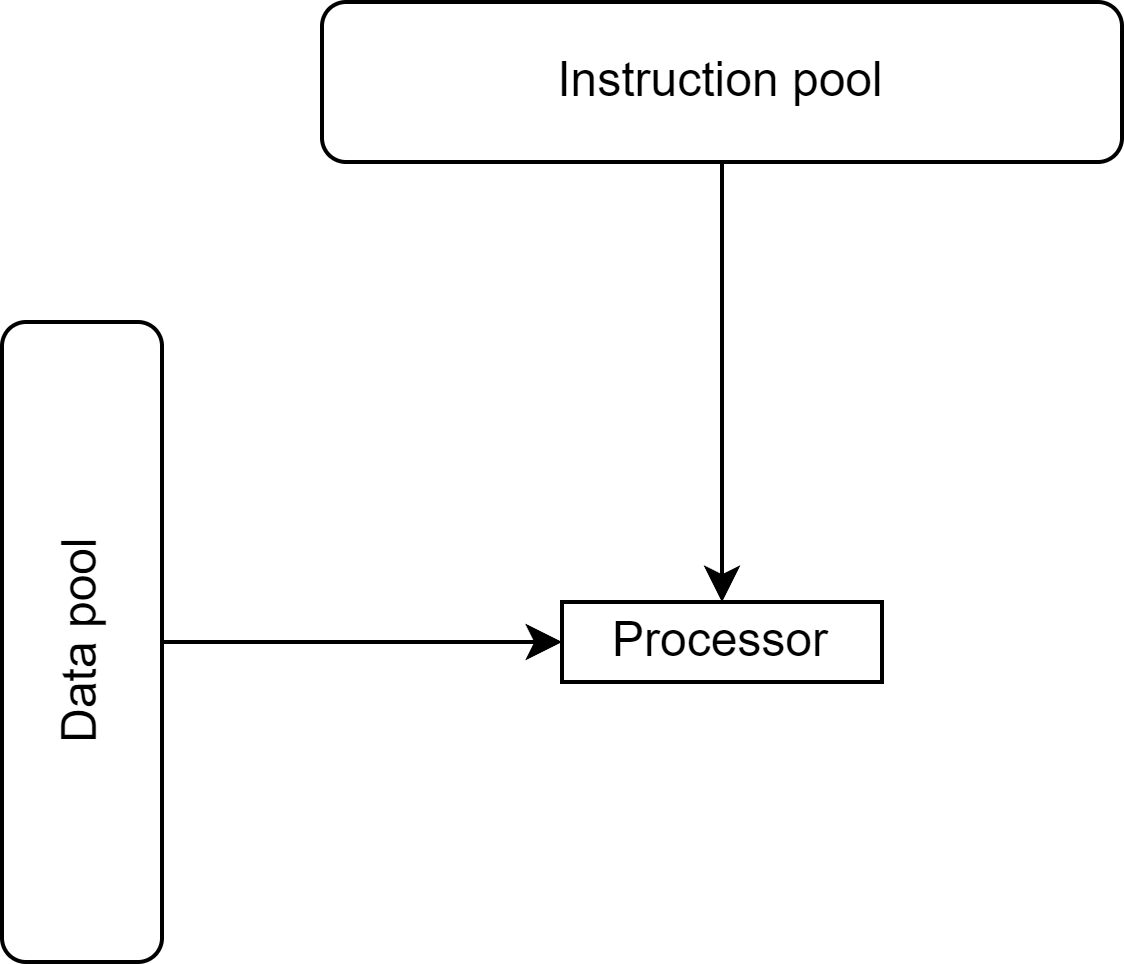
\includegraphics[width=0.3\linewidth]{images/sisd.png}
    \caption{SISD architecture}
\end{figure}
In an SISD architecture, only one instruction is processed by the CPU in each clock cycle, and only one data stream is utilized as input during each clock cycle.
Execution in this setup is deterministic, meaning the outcome is predictable and follows a defined sequence of steps.
SISD architectures represent the most prevalent type of computers.

\subsection{Single Instruction Multiple Data}
In the SIMD architecture, all processing units execute the same instruction simultaneously during each clock cycle, but each processing unit can handle a different data element independently.
This architecture is particularly well-suited for specialized problems with a high level of regularity, such as graphics and image processing.
\begin{figure}[H]
    \centering
    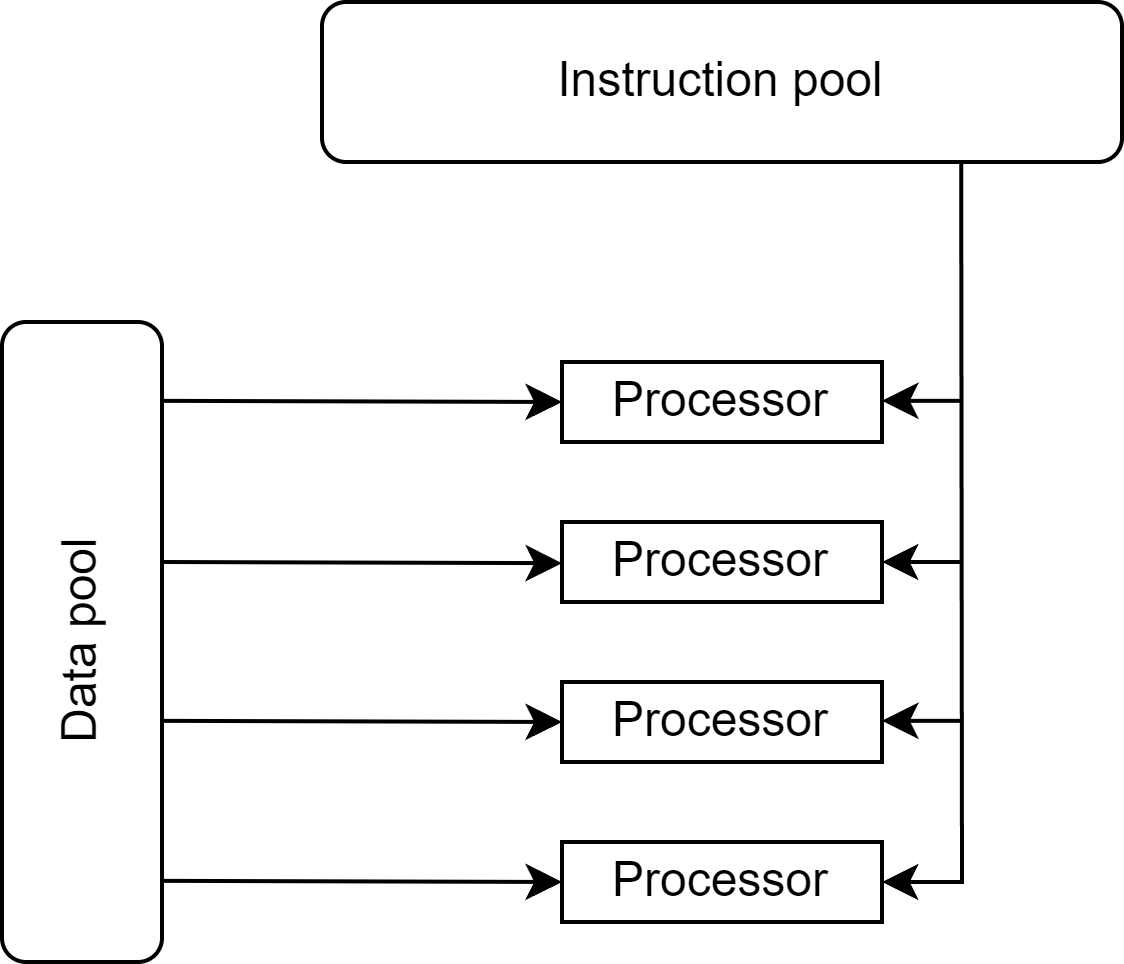
\includegraphics[width=0.3\linewidth]{images/simd.png}
    \caption{SIMD architecture}
\end{figure}

\subsection{Multiple Instructions Multiple Data}
Hardware parallelism can be achieved through various methods:
\begin{itemize}
    \item \textit{Instruction-level parallelism}: this method leverages data-level parallelism at different levels. 
        Compiler techniques such as pipelining exploit modest-level parallelism, while speculation techniques operate at medium levels of parallelism.
    \item \textit{Vector architectures and Graphic Processor Units} (GPU): these architectures utilize data-level parallelism by executing a single instruction across multiple data elements simultaneously.
    \item \textit{Thread-level parallelism}: this approach exploits either data-level or task-level parallelism within a closely interconnected hardware model that enables interaction among threads.
    \item \textit{Request-level parallelism}: this method takes advantage of parallelism among largely independent tasks specified by either the programmer or the operating system.
\end{itemize}
Currently, the most common type of parallel computer features processors that can each execute different instruction streams and operate on distinct data streams. 
Execution in parallel computing can occur synchronously or asynchronously, and it may be deterministic or non-deterministic.
\begin{figure}[H]
    \centering
    \begin{subfigure}{0.49\textwidth}
        \centering
        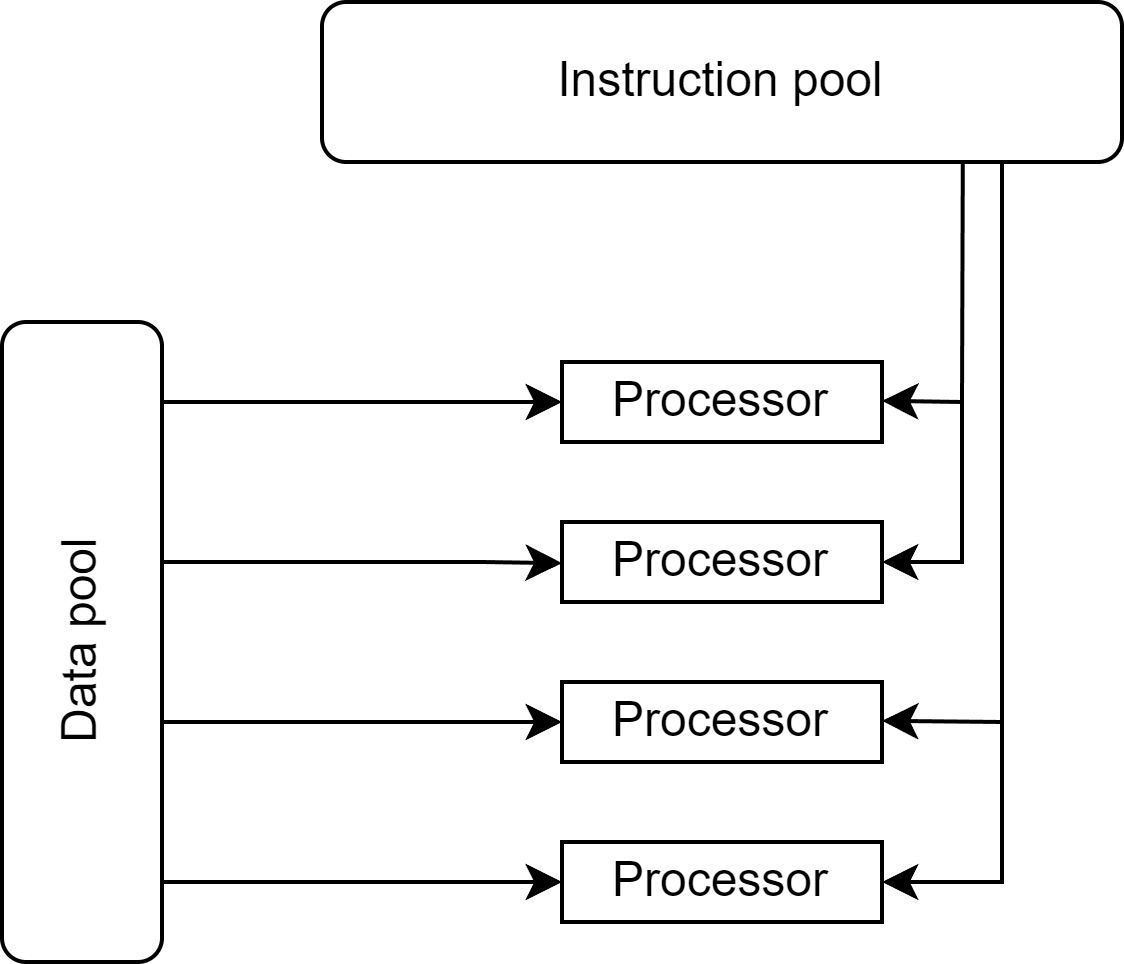
\includegraphics[width=0.6\linewidth]{images/mimd.png} 
        \caption{MIMD architecture}
    \end{subfigure}
    \begin{subfigure}{0.49\textwidth}
        \centering
        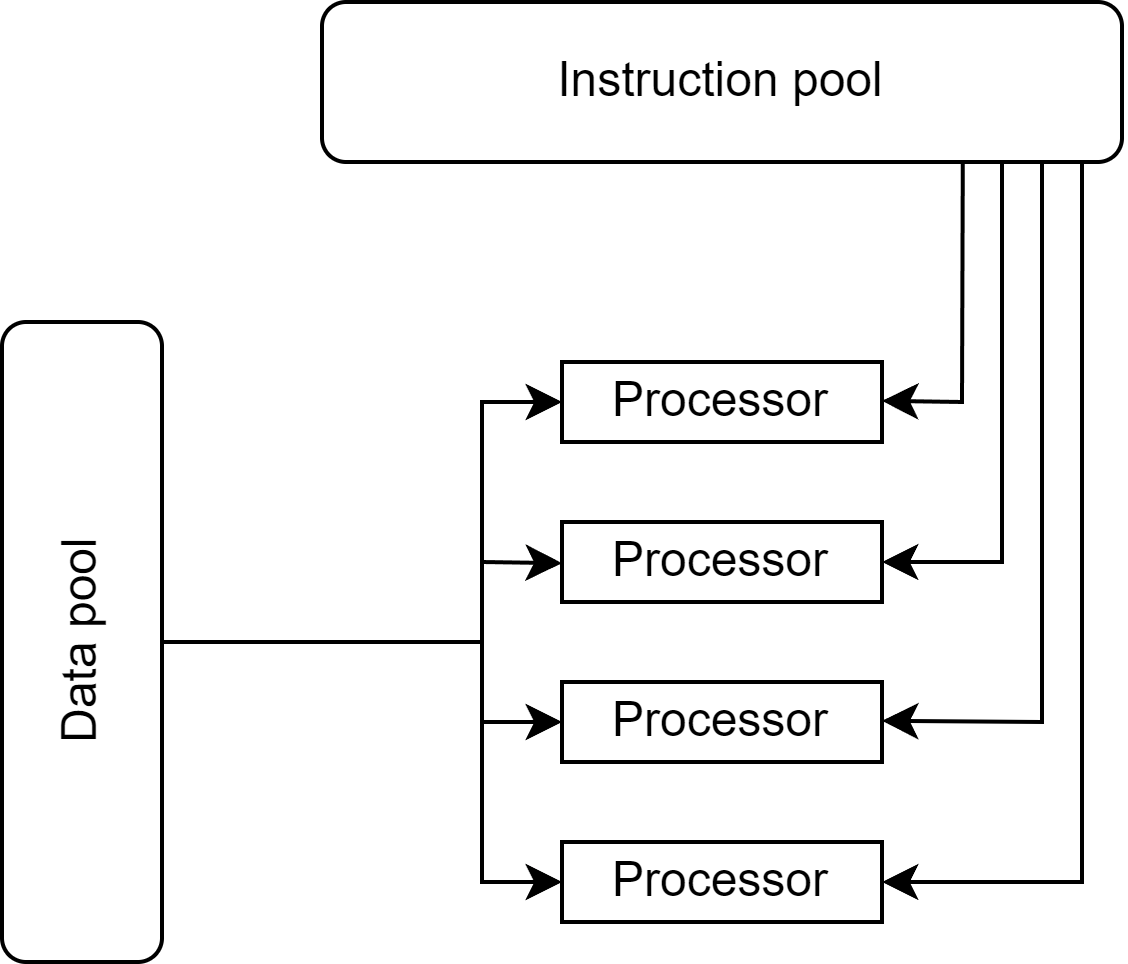
\includegraphics[width=0.6\linewidth]{images/misd.png}
        \caption{MISD architecture}
    \end{subfigure}
    \caption{Possible architectures for hardware parallelism}
\end{figure}